\subsubsection{IronPython}

{\it IronPython} -- реализация языка программирования {\it Python} для платформ {\it .NET Framework} и {\it Mono}. {\it IronPython} полностью написан на {\tt C\#}, и является транслятором компилирующего типа. Код скрипта, написанного на {\it IronPython}, может использоваться одним из следующих способов:
\begin{itemize}
 \item посредством компиляции в независимую сборку, которая в дальнейшем может быть загружена в приложение как зависимось или с помощью {\it .NET Reflection};
 \item посредством размещения {\it IronPython}-подсистемы в основном приложении и динамической трансляции кода.
\end{itemize}

Эта особенность {\it IronPython} очень важна в контексте задач, связанных с автоматизацией ПО.

На схеме, представленной на рисунке \ref{ironpython-scheme}, рассмотрен типичный способ использования {\it IronPython} с целью автоматизации приложения, разрабатываемого для платформы .NET:

\begin{figure}[!h]
    \centering
    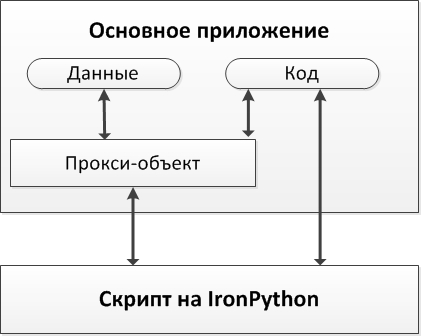
\includegraphics[width=9cm]{ironpython1.jpg}
    \caption{Взаимодействие хост-приложения и скрипта на IronPython}
    \label{ironpython-scheme}
\end{figure}

Для обеспечения взаимодействия скрипта и основного приложения создаётся прокси-объект. Фактически, в этом объекте содержатся ссылки на данные, к которым может осуществляться доступ из скрипта. Теоретически возможен примой доступ к публичным данным хост-приложения, но использовать такую модель не рекомендуется из соображений безопасности и соответствия основным парадигмам объектно-ориентированного приложения. Помимо данных, скрипт может использовать код (классы и функции), реализованный в хост-приложении.